% -*- TeX-master: "paper.tex"; TeX-PDF-mode: t; ispell-local-pdict: "words" -*-

%%%%%%%%%%%%%%%%%%%%%%%
%%%% Figures %%%%%%%%%%
%%%%%%%%%%%%%%%%%%%%%%%

\begin{figure}
\centerline {
%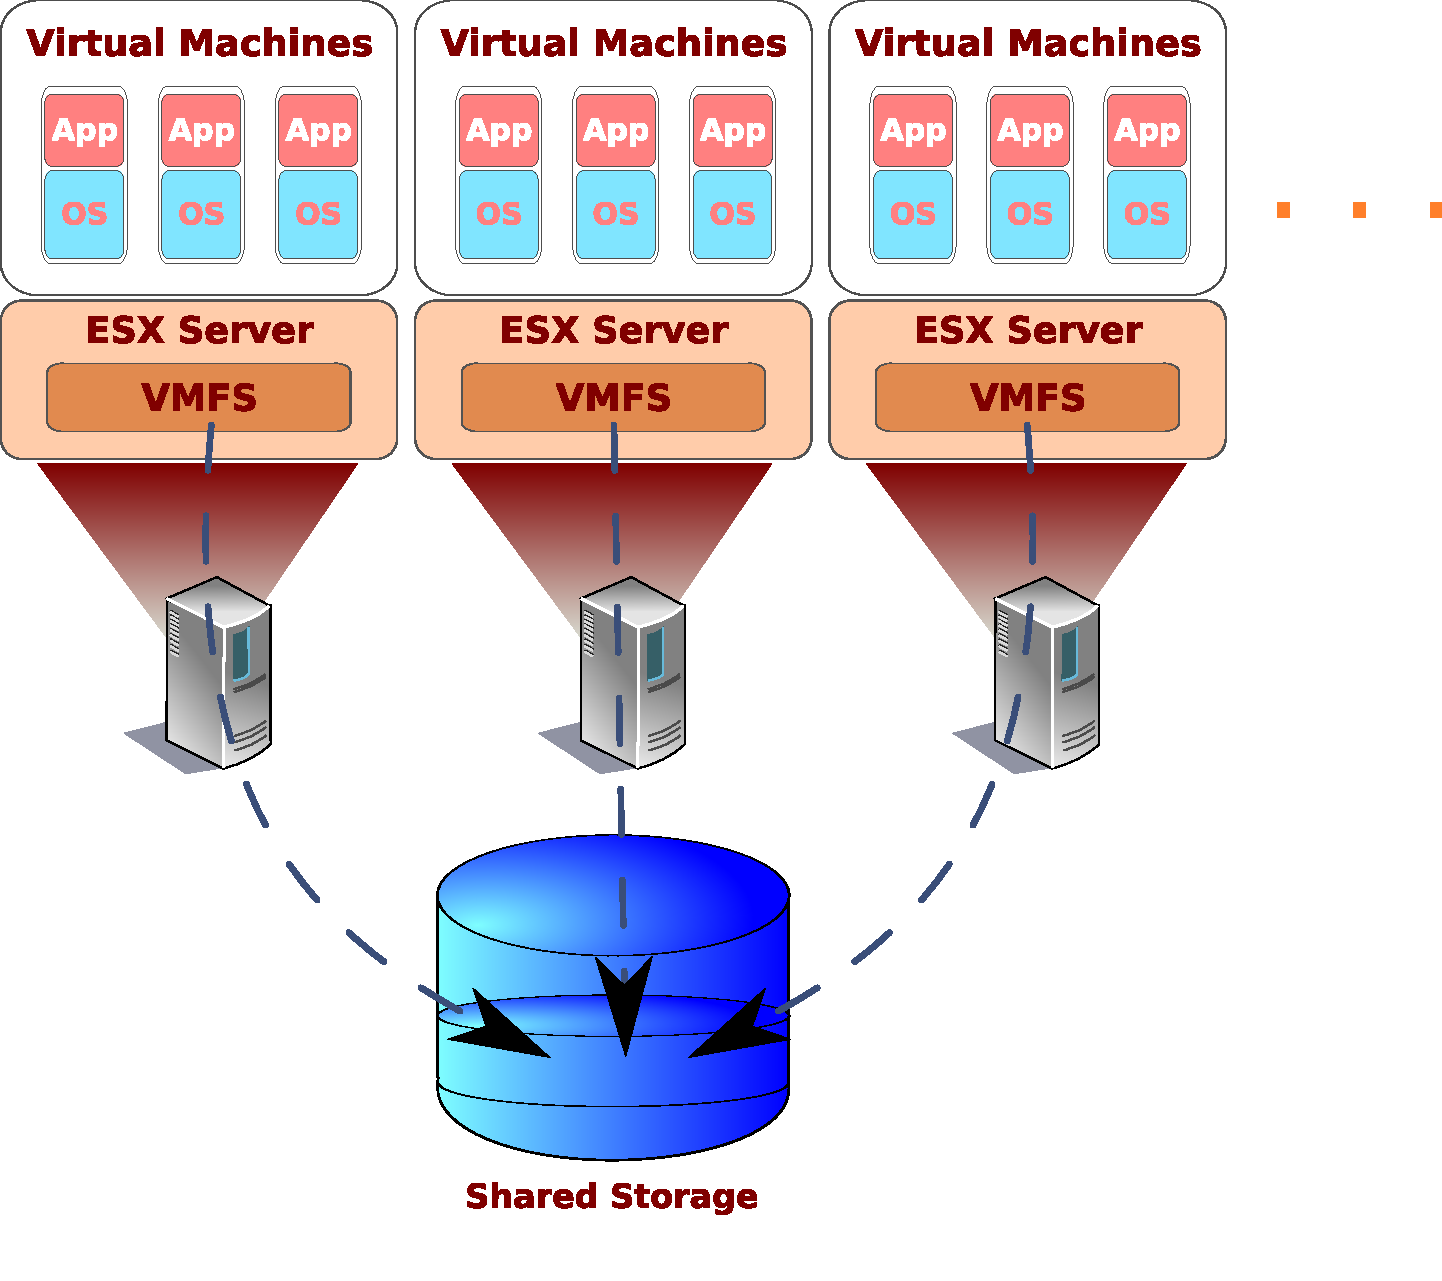
\includegraphics[width=70mm]{figures/vmfs_sysmodel.pdf}
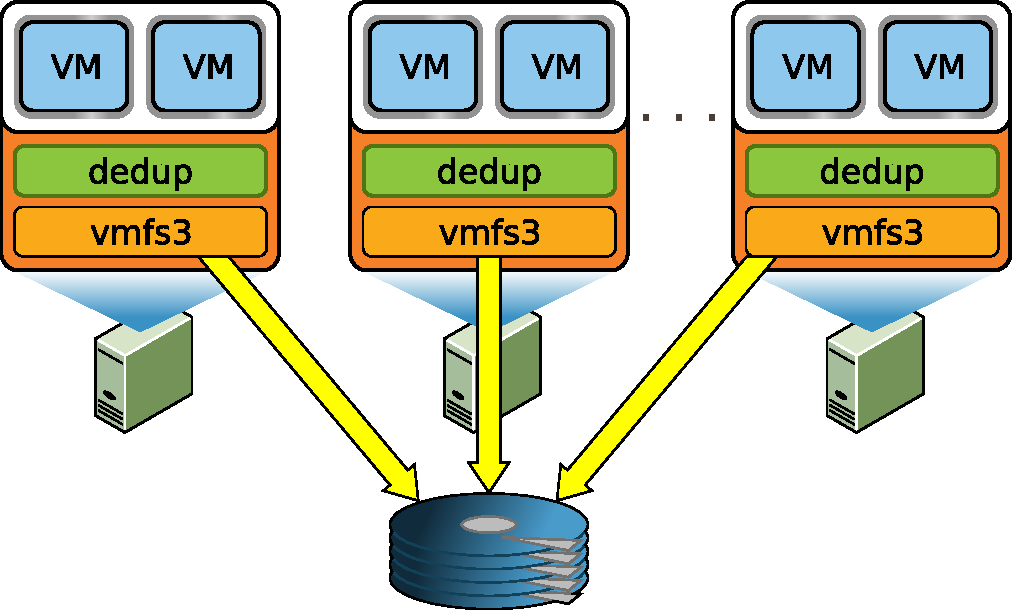
\includegraphics[scale=0.45]{figures/vmfs.pdf}
}
%\vspace{-0.2in}
\caption{Cluster configuration in which multiple hosts
  concurrently access the same storage volume.  Each host runs the
  VMFS file system driver ({\tt \small vmfs3}), the deduplication
  driver ({\tt \small dedup}), and other
  processes such as VMs.}
%\vspace{-0.1in}
\label{fig:vmfs-sysmodel}
\end{figure}


\section{System Overview}
\label{sec:overview}
\label{sec:idea:out-of-band}

\DeDe operates in a cluster setting, as shown in
Figure~\ref{fig:vmfs-sysmodel}, in which multiple hosts are directly
connected to a single, shared SCSI volume and use a file system designed
to permit symmetric and cooperative access to the data stored on the
shared disk.  \DeDe itself runs on each host as a layer on top of the
file system, taking advantage of file system block layout policies and
native support for copy-on-write (COW) blocks.  In this section, we
provide a brief overview of our approach to deduplication and the file
system support it depends on.

% Content hash index

\DeDe uses content hashes to identify potential duplicates,
the same basic premise shared by all deduplication systems.  An index
stored on the shared file system and designed for concurrent access
permits efficient duplicate detection by tracking all known blocks in
the file system by their content hashes.

% Overall scheme

%% As a sketch, file system write operations are intercepted by \DeDe and
%% content hashes are computed while the IO is still in memory. This
%% summary data, called a write log, which constitutes the file system
%% modifications for a particular host is accumulated on each host
%% independently and periodically flushed to the shared disk. Later on,
%% the write log is compared against the deduplication index when, if
%% duplicates are discovered, we can create merge requests to eliminate
%% duplication. These merge requests are in turn, handled by a multitude
%% of hosts independently and asynchronously.

% Out of band

In order to minimize impact on critical file system operations such as
reading and writing to files, \DeDe updates this index \emph{out of
  band}, buffering updates and applying them in large, periodic
batches.  As part of this process, \DeDe detects and eliminates
duplicates introduced since the last index update.  This can be
done as an infrequent, low priority
background task or even scheduled during times of low
activity.  Unlike approaches to deduplication such as
content-addressable storage that integrate content indexes directly
into the file system storage management, \DeDe's index serves solely to
identify duplicate blocks and plays no role in general file system
operations.

\DeDe divides this index update process between hosts.  Each host
monitors its own changes to files in the cluster file system and
stores summaries of recent modifications in on-disk \emph{write logs}.
These logs include content hashes computed in-band, as blocks are
written to disk.  Each host periodically consumes the write logs of files
it has (or can gain) exclusive access to and updates the shared index
\XXX[under exclusive lock] to reflect these recorded modifications. In
the process, it discovers and reclaims any block whose content is
identical to the content of some previously indexed block.  Having
each host participate in the index update process allows the hosts to
divide and distribute the burden of deduplication, while sharing the
index allows hosts to detect duplicates even if they are introduced by
separate hosts. \XXX[Irfan][REVIEW the last line.]

% Resilience

Out-of-band index updates mean \DeDe must be resilient to stale index
entries that do not reflect the latest content of recently updated
blocks.  Indeed, this is essentially unavoidable in a decentralized
setting because of communication delays alone.  While this means \DeDe
generally must verify block contents when updating the index, this
resilience has an important implication: \DeDe's correctness does not
depend on its ability to monitor every write to the file system.  This
has important performance benefits.  First, updates to write logs do
not have to be crash-consistent with updates to file contents, which
both simplifies fault tolerance and allows hosts to buffer updates to
write logs to minimize additional IO.  Second, this allows users to
trade off the CPU and memory overhead of write
monitoring for peak file system performance on a per-file basis.  For
example, a user could simply disable deduplication for VMs that are
performance-critical or unlikely to contain much duplicate data.
Finally, this allows the write monitor to shed work if the system is
overloaded.

% Unique blocks

Because \DeDe operates on a live file system, it specifically
optimizes for \emph{unique} blocks (blocks with no known duplicates).
Unlike \emph{shared} blocks, these blocks remain mutable after
deduplication.  The mutability of unique blocks combined with \DeDe's
resilience to stale index information means these blocks can be
updated in place without the need to allocate space for a copy or to
synchronously update the index.  As a result, deduplication has no
impact on the performance of writing to unique blocks, a highly
desirable property
because these are precisely the blocks that do not benefit from
deduplication.

Similar to some other deduplication work related to virtual
disks~\cite{cas-experiences,nath08hpccas}, \DeDe uses fixed-size
blocks.  Unlike stream-oriented workloads such as backup, where
variable-sized chunks typically achieve better
deduplication~\cite{zhu08datadomain}, our input data is expected to be
block-structured because guest file systems (\eg, ext3, NTFS)
typically divide the disk into fixed-size 4~KB or 8~KB blocks
themselves.  Consistent with this expectation, earlier
work~\cite{nath06vmcas} and our own test results (see
Section~\ref{sec:vmware-vdi-analysis}), we use a block size of 4~KB.

\subsection{Required File System Abstractions}
\label{sec:idea:compare-and-share}

Most approaches to deduplication unify duplicate elimination and
storage management, supplanting the file system entirely.  \DeDe, in
contrast, runs as a layer on top of VMFS, an existing file system.
This layer finds potentially identical blocks and identifies them to
the file system, which is then responsible for merging these blocks
into shared, copy-on-write blocks.

\XXX[Austin][Better transition?]
\DeDe requires the file system to be block oriented and to support
file-level locking.  The file
system block size must also align with the deduplication block size, a
requirement VMFS's default 1~MB block size, unfortunately, does not
satisfy.  Our only non-trivial change to VMFS was to add support for
typical file system block sizes (\ie, 4~KB), as detailed later in
Section~\ref{sec:vmfs}.

Finally, \DeDe requires block-level copy-on-write support, a well
understood, but nevertheless uncommon feature supported by VMFS.
Specifically, it requires an unusual \emph{compare-and-share} operation,
which replaces two blocks with one copy-on-write block after verifying
that the blocks are, in fact, identical (using either bit-wise
comparison or a content hash witness).  Despite the specificity of
this operation, it fits naturally into the structure of block-level
copy-on-write and was easy to add to the VMFS interface.  \DeDe
manipulates file system blocks solely through this interface and has
no knowledge of the underlying file system representation.

There are two noteworthy capabilities that \DeDe does \emph{not}
require of the file system.  First, hosts running \DeDe never modify
the metadata of files they do not have exclusive locks on, as doing so
would require cross-host synchronization and would complicate per-host
metadata caching.  As a result, a host that discovers a duplicate block
between two files cannot simply modify both files to point to the
same block if one of the files is locked by another host.  Instead,
when \DeDe detects a duplicate between files locked by different
hosts, it uses a third file containing a \emph{merge request} as an
intermediary.  One host creates a merge request containing a COW
reference to the deduplicated block, then passes ownership of the
merge request file's lock to the other host, which in turn replaces
the block in its file with a reference to the block carried by the
merge request.

% Section 2.1, 3rd paragraph, last sentence, mentions and italicizes
% merge requests, but doesn't define them (they're described later in
% 2.2).  If you're going to emphasize them, you may as well provide some
% kind of definition or forwarding pointer.

Second, \DeDe does \emph{not} require the file system to expose a
representation of block addresses.  Much like any regular application,
it only refers to blocks indirectly, by their offset in some
locked file, which the file system can resolve into a block
address.  This restricts the design of our index, since it cannot
simply refer to indexed blocks directly.  However, this limitation
simplifies our overall design, since requiring the file system to expose block
addresses outside the file system's own data structures would
interfere with its ability to free and migrate blocks and could result
in dangling pointers.  Worse, any operations introduced to manipulate
blocks directly would conflict with file-level locking and host
metadata caching.

In lieu of referring to blocks by block addresses, \DeDe introduces a
\emph{virtual arena} file.  This is a regular file in the file system,
but it consists solely of COW references to shared blocks that are
present in at least one other file.  This file acts as an alternate
view of all shared blocks in the system: \DeDe identifies shared
blocks simply by their offsets in the virtual arena file, which the
file system can internally resolve to block addresses using regular
address resolution.

Because \DeDe builds on the underlying file system, it inherits the
file system's block placement policy and heuristics.  If the
underlying file system
keeps file blocks sequential, blocks will generally remain sequential
after deduplication.  Shared blocks are likely to be sequential with
respect to other blocks in at least one file, and common sequences of
shared blocks are likely to remain sequential with respect to each
other.  Furthermore, the placement and thus sequentiality of unique
blocks is completely unaffected by the deduplication process; as a
result,
%
% not only is IO performance to individual unique blocks
% unaffected after deduplication because they do not require copying,
% but sequential IO performance across spans of unique blocks is also
% maintained.
%
deduplication does not affect IO performance to individual unique
blocks because they do not require copying, and it maintains
sequential IO performance across spans of unique blocks.

\subsection{VMFS}
\label{sec:vmfs}

Many of the design decisions in \DeDe were influenced by the design of
its substrate file system, VMFS.  VMFS is a coordinator-less cluster
file system~\cite{vmfsdatasheet} designed to allow hosts to
cooperatively maintain a file system stored on a shared disk. In this
section, we provide a quick overview of how VMFS addresses and
manages concurrent access to its resources in order to provide better
context for the design of \DeDe.

VMFS organizes the shared disk into four different resource pools:
inodes, pointer blocks, file blocks, and sub-blocks.  Inodes and
pointer blocks play much the same role as in traditional UNIX file
systems, storing per-file metadata and pointers to the blocks
containing actual file content.  File blocks and sub-blocks both store
file content, but are different sizes, as discussed below.  The
divisions between these pools are currently fixed at format time and
can only be expanded by adding more storage, though this is not a
fundamental limitation.  In each pool,
resources are grouped into \emph{clusters}. The header for each cluster
maintains metadata about all of its contained resources; most
importantly, this includes a reference count for each
individual resource and tracks which resources are free and which are
allocated.

In order to support concurrent access by multiple hosts to file and
resource data, VMFS uses a distributed lock manager.
Unlike most cluster file systems, which use an
IP network for synchronization, VMFS synchronizes all file system
accesses entirely through the shared disk itself using on-disk locks.
VMFS ensures atomic access to on-disk lock structures themselves using
SCSI-2-based LUN reservations to guard read-modify-write critical
sections.  In addition to taking advantage of the reliability of
storage area networks, using the same means to access both file system
state
and synchronization state prevents ``split brain'' problems typical of
IP-based lock managers in which multiple hosts can access the file
system state but cannot communicate locking decisions with each other.

VMFS protects file data from concurrent access by associating a
coarse-grain lock with each file that covers all of a file's metadata
(its inode and pointer blocks) as well as all of the file blocks and
sub-blocks comprising the file's content.  Files in VMFS tend to be
locked for long durations (\eg, a VM's disk files are locked as long
as the VM is powered on). \DeDe respects file system locking by
partitioning the deduplication process according to which hosts hold
which file locks.
% ... so \DeDe must deduplicate data blocks in locked files in a
% manner that is both efficient and respects the file system locking
% protocol.

VMFS protects resource metadata using per-cluster locks.  Thus,
allocation and deallocation of resources must lock all clusters
containing any of the resources involved.  The number of resources
packed per cluster reflects a trade-off between locking overhead and
cross-host cluster lock contention.  Higher cluster density allows
hosts to manipulate more resources with fewer locks, but at the cost of
increased lock contention.  Since \DeDe stresses the sub-block resource pool
more than typical VMFS usage, we increase the sub-block cluster
density from 16 to 128 resources per cluster, but otherwise use the
default VMFS densities.

% JL: agree, removed
% \XXX[Austin][This is probably good to talk about, but doesn't fit in
% very nicely.]
% Resource allocation in VMFS is similar to that of a next-fit memory
% allocator~\cite{next-fit}.  Each host uses a hash of its own MAC
% address to pick an initial cluster from which to allocate resources
% when mounting the file system.  The host allocates from this cluster
% until exhausting it and moving on to the next cluster.  The staggering
% of initial allocation clusters combined with lingering until clusters
% are exhausted helps to minimize cross-host lock contention, but can
% negatively impact sequentiality.

\begin{figure}[t]
\centerline {
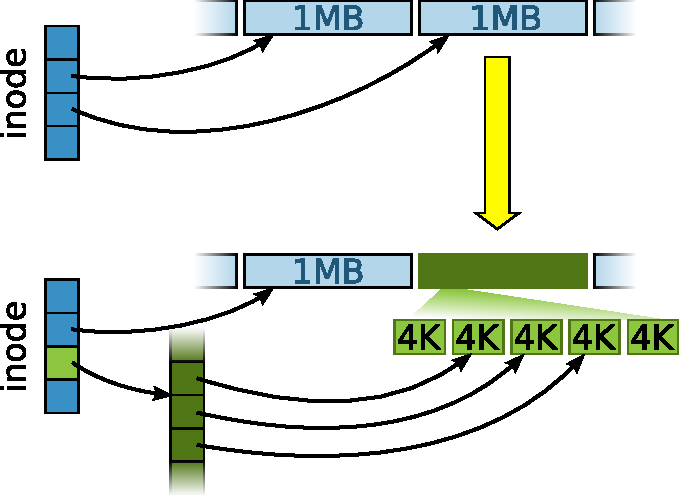
\includegraphics[scale=0.45]{figures/mixed.pdf}
}
\caption{Mixed block sizes allow any 1~MB file block to be divided into
  256 separate 4~KB sub-blocks.}
\label{fig:mixed-block-sizes}
\end{figure}

VMFS maintains two separate resource types for storing file content:
file blocks and sub-blocks.  File sizes in VMFS typically fit a
bimodal distribution.  Virtual machine disks and swap files are
usually several gigabytes, while configuration and log files tend to
be a few kilobytes.  Because of this, VMFS uses 1~MB file blocks to
reduce metadata overhead and external fragmentation for large files,
while for small files, VMFS uses smaller
sub-blocks to minimize internal fragmentation.
\DeDe must be able to address individual 4~KB blocks in order to COW
share them, so we configure VMFS with 4~KB sub-blocks.
Furthermore, rather than simply eschewing the efficiency of 1~MB blocks
and storing all file content in 4~KB blocks, we extend VMFS to
support \emph{mixed block sizes}, depicted in
Figure~\ref{fig:mixed-block-sizes}, so that \DeDe can address
individual
4~KB blocks of a file when it needs to share a duplicate block, but
when possible still store unique regions of files in efficient 1~MB
blocks.  This change introduces an optional additional pointer block
level and allows any file block-sized region to be broken into 256 
separate 4~KB blocks, which, in turn, add up to the original file
block.  This can be done
dynamically to any 1~MB block based on deduplication decisions,
and leaves address resolution for other data intact and efficient.

Beyond these unusual block sizes, VMFS supports a number of other
uncommon features.  Most important to \DeDe is support for block-level
copy-on-write (COW).  Each file or sub-block resource can be
referenced from multiple pointer blocks, allowing the same data to be
shared between multiple places in multiple files.  Each reference to a
shared resource is marked with a COW bit, indicating that any attempts
to write to the resource must make a private copy in a freshly
allocated resource and write to that copy instead.  Notably, this COW
bit is associated with each \emph{pointer} to the resource, not with the
resource itself.  Otherwise, every write operation would need to take
a cluster lock to check the COW bit of the destination block, even if
the block was not COW.  However, as a result, sharing a block between
two files requires file locks on \emph{both} files, even though only
one of the references will change.  Thus, \DeDe must use merge
requests for all cross-host merging operations.

VMFS forms the underlying substrate of \DeDe and handles critical
correctness requirements such as specializing COW blocks and
verifying potential duplicates, allowing \DeDe to focus on
duplicate detection.  Virtual arenas and merge requests
allow \DeDe to achieve complex, decentralized manipulations of the
file system structure without knowledge of the file system
representation, instead using only a few general-purpose interfaces.

% VMFS has attained significant market acceptance with a majority of
% VMware ESX Server users deploying it in their environments to run
% enterprise production workloads. As such, VMFS provided a well-tested
% base to develop our \DeDe prototype on top of.

% Each system file has a resource file header, followed by multiple
% recurring sequences of densely packed resource clusters (along with
% their associated disk locks) and the resources they are comprised of.
% The resource file header describes the number of resources per
% cluster, number of clusters per cluster group, size of each resource,
% total number of resources and cluster groups and other information
% needed to manage the specific resource type.  The resource clusters
% have a resource bitmap to track resource allocation and deallocation
% and a two byte reference counter per resource to track the total
% number of references to a specific resource (which is used to
% implement snapshots). Resources are deallocated and marked free in the
% bitmap only when their corresponding reference counters drop to zero.

% The inode structure in VMFS is akin to that of a traditional UNIX file
% system inode with pointers to fixed-size blocks. Due to the fairly
% large file block sizes, the design does not support more than a
% single-level of indirection via pointer-blocks
% (Section~\ref{sec:mixed-block-sizes} describes why this limitation had
% to be overcome for \DeDe).  As a performance optimization, VMFS embeds
% the copy-on-write flag in the file metadata itself instead of the
% block metadata. This implies that even if modifying file A to point to
% a block in file B, a lock might still be needed on file B to make its
% pointer COW.  Another important design aspect that has performance
% implications for copy-on-write with VMFS (and \DeDe) is the fact that
% resource clusters (block metadata) do not hold a back reference to the
% holder(s) of the resource (file metadata). This implies that if there
% are two copy-on-write references to the same block from file A and
% file B, deletion of file B will not automatically cause the
% copy-on-write flag in file A's metadata to be unset. A subsequent
% write will still incur the penalty of a copy-on-write.

% \subsection{Content Hashing}
% \label{sec:content-hashing}

% \DeDe uses \shaone~\cite{fips-180-2} to fingerprint contents of
% blocks. To date, there aren't any known hash collisions from using the
% \shaone function and it is generally considered a collision-resistant
% crypto secure hash. However, there is debate about whether history
% will repeat itself with this function eventually getting broken in a
% computationally feasible implementation~\cite{henson-compare-by-hash,
%   black-compare-by-hash}. Whereas we hold that using \shaone or similar
% function is safe for our purposes, we chose to keep the flexibility in
% \DeDe to perform bit-by-bit comparisons before deduplicating. It is
% worth noting that the \shaone hashes are used in our system to simply
% identify duplicates and not to address them during normal
% runtime. \DeDe only supports traditional file system location
% addressing using the $\tup<\text{filename},\text{offset}>$ tuple. As
% such, if \shaone must be replaced, our system can be safely
% upgraded by installing a new hash function and reconstructing the
% index, a process during which the file system can continue to execute
% without interruption.

%% a worst-case workload for \DeDe is encrypted guest fileystems,
%% nevertheless \DeDe can provide good deduplication peformance for a
%% variety of workloads.



